\xiti
\begin{xiaotis}

\xiaoti{用刻度曲尺检查长方体形工件的相对两个面是否平行,你能想出几种方法?}

\xiaoti{三个平面有公共点,说这些平面有公共直线对吗?当这些平面两两相交时,可以得到几条交线。}

\xiaoti{}%
\begin{xiaoxiaotis}%
    \xxt[\xxtsep]{以已知平面内不在同一条直线上的三点为端点,在平面的同一侧分别引三条平行且相等的线段。
        求证:过另外三个端点的平面与已知平面平行。
    }

    \xxt{在共点 $O$ 的三条不共面直线 $a$、$b$、$c$ 上,在点 $O$ 的两侧分别取点 $A$ 和 $A'$、$B$ 和 $B'$、$C$ 和 $C'$,
        且 $AO = A'O$、$BO = B'O$、$CO = C'O$。求证:$\text{平面}\;ABC \pingxing \text{平面}\; A'B'C'$。
    }

\end{xiaoxiaotis}

\xiaoti{\zhongdian{经过平面外一点只有一个平面和已知平面平行。}}

\xiaoti{}%
\begin{xiaoxiaotis}%
    \xxt[\xxtsep]{如果一条直线和两个平行平面中的一个相交,那么它和另一个也相交;}

    \xxt{如果一个平面和两个平行平面中的一个相交,那么它和另一个也相交;}

    \xxt{平行于同一个平面的两个平面平行。}

\end{xiaoxiaotis}


\xiaoti{一条直线和两个平行平面相交。求证:它和两个平面所成的角相等。}

% TODO: wrapfigure 在这里无法正常使用
\begin{minipage}{10.5cm}
    \jiange

    \xiaoti{两个平行平面的距离等于 12 cm,一条直线和它们相交成 $60^\circ$ 角,求这条直线上夹在这两个平面间的线段的长。}

    \xiaoti{$a$ 和 $b$ 是两条异面直线。 求证:过 $a$ 且平行于 $b$ 的平面必平行于过 $b$ 且平行于 $a$ 的平面。}

    \begin{enhancedline}

    \xiaoti{如图,直线 $AC$、$DF$ 被三个平行平面 $\alpha$、$\beta$、$\gamma$ 所截。求征:
        $$\dfrac{AB}{BC} = \dfrac{DE}{EF} \juhao $$
    }

    \xiaoti{过已知平面外一点且平行于该平面的直线,都在过已知点平行于该平面的平面内。}
    \end{enhancedline}

\end{minipage}
\quad
\begin{minipage}{4cm}
    \centering
    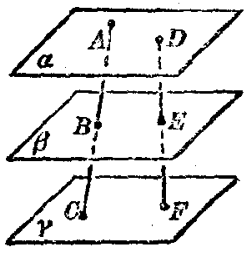
\includegraphics[width=4cm]{../pic/ltjh-ch1-xiti5-09.png}\\
    (第 9 题)

\end{minipage}
\vspace{1em}

\end{xiaotis}

